
\section{{\feff}}


\subsection{Scattering Amplitude and Phase}
\begin{frame} \frametitle{Scattering Amplitude and Phase-Shift:
    ${f(k)}$ and ${\delta(k)}$ }

  The scattering amplitude ${\Red{f(k)}}$ and phase-shift
  ${{\Red{\delta(k)}}}$ depend on Z:

    \vmm

    \begin{tabular}{ll}
      \begin{minipage}{55mm}
        \rgraph{55mm}{scatt_amp}
        \end{minipage} &
        \begin{minipage}{55mm}
          \rgraph{55mm}{scatt_pha}
      \end{minipage}\\

      \begin{minipage}{55mm}
      $\Red{f(k)}$ peaks at higher  $k$ as Z increases.  Heavy
        elements, have a characteristic dip in $\Red{f(k)}$, and
        scatter to high $k$.  

        {\bf{Note: O is done at $k>15\rm\AA^{-1}$}}


      \end{minipage}
      &
      \begin{minipage}{55mm}

        The phase shift $\Red{\delta(k)}$ also shows strong Z
        dependence, and has sharp jumps for heavy elements where $f(k)$ dips.

        {\bf{Note:  $\delta(k) \approx -k$! }}
      \end{minipage} \\
    \end{tabular}

\begin{postitbox}{50mm}
  Z can usually be determined to $\pm 5$.

\vmm
  Fe and O can be distinguished.

\vmm
  N  and O cannot be distinguished.
\end{postitbox}
\vfill
\end{frame}


\begin{frame} \frametitle{ $\lambda(k)$: The Photo-Electron Mean-Free Path }

 \begin{cenpage}{102mm}
  The $ e^{-2R/\lambda(k)} $ term in the XAFS Equation accounts for how far the
   photo-electron can travel and still return (in phase) to the excited atom.
 \begin{columns}
   \begin{column}{55mm}
     \rgraph{57mm}{lambda}
   \end{column}
   \begin{column}{60mm}

     This includes both:

     \begin{itemize}
     \item  inelastic scattering of photo-electron.
     \item  finite lifetime of the core-hole (fs).
     \end{itemize}
     \vmm

   \end{column}
 \end{columns}

 \vmm\hrule\vmm

Basically, the photo-electron can only go out 20 \AA or so over most of the
EXAFS region. 

 \begin{postitbox}{80mm}
     The $\lambda$ and $1/R^{2}$ terms make EXAFS a  {\RedEmph{local probe}}.
   \end{postitbox}

  \end{cenpage}
\end{frame}


\subsection{{\feff}}
\begin{frame}
  \frametitle{{\feff} Calculation Overview}

  \begin{cenpage}{112mm}
  {\feff} calculates the EXAFS {$\chi(k)$}  by simulating the scattering of a
  photo-electron along all scattering paths from a selected absorbing atom within
  a  cluster of atoms.
  \end{cenpage}

  \vmm
  
  \begin{enumerate}
    \onslide+<2->\item   build atomic potentials.   To  simplify calculations,

      \begin{center}
        \begin{tabular}{ll}
          \begin{minipage}{80mm}
            Use the {\BlueEmph{Cup-Cake Tin Approximation}}:
            atomic potentials up to a uniform Fermi level -no chemical bonding.

            \hspace{4mm}(Sometimes called ``Muffin-Tin'' Approximation)
          \end{minipage}
          &
          \begin{minipage}{25mm}
            \vspace{1mm} 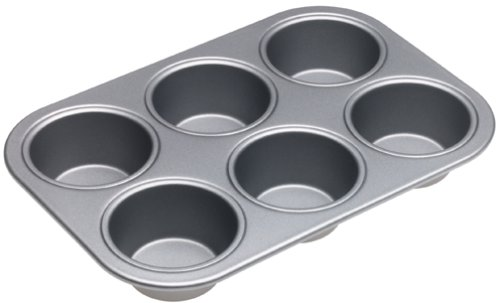
\includegraphics[width=20mm]{figs/theory/muffintin2}
          \end{minipage}
        \\
      \end{tabular}
    \end{center}


  \onslide+<3->\item determine important scattering paths.

    \begin{itemize}
    \item Build paths from a selected {\BlueEmph{central atom}} in a cluster of atoms
    \item decide which ones are ``degenerate'' .
    \item decide which ones are unimportant for XAFS
    \end{itemize}


  \onslide+<4->\item move photo-electron along path to determine
    $\Red{f}$ and $\Red{\delta}$ as a function of $k$:

    \begin{center}
      propagate $\Rightarrow$ scatter $\Rightarrow$ propagate $\Rightarrow$ \ldots.
    \end{center}

  \end{enumerate}

\end{frame}

\subsection{{\feff}   complications}
\begin{frame} \frametitle{{\feff}: what's so hard about that??}

  \begin{cenpage}{105mm}
    {\feff} includes sophisticated techniques to calculate of \feffc{f(k)},
    \feffc{\delta(k)}, and \feffc{\lambda(k)}.

    \begin{description}
    \item[\RedEmph{Curved Wave Effects}] the photo-electron goes out as
      spherical wave and scatters from atoms with finite size.

    \item[\RedEmph{Muffin-Tin Approximation:}] Makes the calculations
      tractable, but is an approximation.

    \item[\RedEmph{Multiple Scattering}]  the photo-electron can scatter
      multiple times. Most important at low $k$ and for \BlueEmph{linear paths}.

    \item[\RedEmph{Extrinsic Losses}] {\feffc{\lambda(k)}}: self-energy and
      core-hole lifetime.

    \item[\RedEmph{Intrinsic Losses}] {\feffc{S_0^2}}: the absorbing atom
      relaxes to the presence of the hole left in the core electron level.

    \item[\RedEmph{Polarization Effects}] synchrotron beams are highly
      polarized, which needs to be taken into account.  This is simple for
      $K$ edges ($s\rightarrow p$ is dipole), but slightly more complicated for
      $L$ and $M$ edges.

    \end{description}

    \end{cenpage}
\vmm
\begin{center} Usually, you don't have to worry about these things!\end{center}

\end{frame}


\section{{\feff} complications}

\subsection{{\feff} complication \#1: Multiple Scattering}
\begin{frame} \frametitle{{\feff} complication \#1: Multiple Scattering}

  \vmm
\begin{columns}
  \begin{column}{50mm}
  The photo-electron can scatter multiple times before getting back to the
  absorbing atom:

  \begin{center}
    \rgraph{50mm}{mspaths}
  \end{center}

  \end{column}
  \begin{column}{60mm}

  A {\Blue{Path Formalism}} is used in the  calculation:

  \begin{center}
    propagate $\Rightarrow$ scatter $\Rightarrow$ propagate $\Rightarrow$ \ldots.
  \end{center}

  \vmm  \pause
  \vmm {\Red{Single Scattering}}  usually important.

  \vmm {\Red{Triangle Paths}} with angles $ 45 < \theta <
  135^{\circ}$ scatter weakly, but there are lots of them.

  \vmm {\Red{Linear paths}} with angles $\theta \approx 180^{\circ}$
   are very strong: the photo-electron is {\Red{focused}} through an atom.
   Can be used to measure bond angles\ldots

  \end{column}
  \end{columns}

   \begin{postitbox}{92mm}
     \Red{ A {\feff} Path looks the same for Single and Multiple
       Scattering}
   \end{postitbox}
\end{frame}

\subsection{{\feff} Complication \#2: S02}
\begin{frame} \frametitle{{\feff} complication \#2: $S_0^2$, the  Amplitude Reduction Term}

  \vmm
    \begin{cenpage}{110mm}

  The {\RedEmph{other}} electrons in the absorbing atom can relax due to
  the core-hole, giving an {\Red{Amplitude Reduction Term}}:

   \vmm
   \[
   S_0^2 =  {  |{\langle \Phi^{N-1}_f |\Phi^{N-1}_0 \rangle}|^2}
   \]

    \vspace{1mm}

    ${| \Phi^{N-1}_0 \rangle }$ = $(N-1)$ electrons in unexcited atom.

    ${\langle \Phi^{N-1}_f|}$   = $(N-1)$ electrons, relaxed by core-hole.

    \vmm

    \onslide+<2->
    ${S_0^2}$ is taken as a constant: \hspace{3mm}  $ 0.7 < S_0^2 < 1.0 $.

    and may be used as a Fitting Parameter that multiplies {$\chi$}:

    \vmm \vmm
    \onslide+<3->
    \begin{center}
      {\Red{ ${S_0^2}$ is Completely Correlated with $N$      (!!!)}}
    \end{center}

    \onslide+<4->

    \begin{postitbox}{68mm}
      $S_0^2$ is usually constant for  data measured on
      the same edge {\bf{and}} beamline (energy resolution).
    \end{postitbox}

    Most Common Approach: Determine $S_0^2$ from experimental data on a
    system with known $N$, and then use that for unknown data. 

    \vmm

    \end{cenpage}

\end{frame}
